\FloatBarrier
\subsection{LS identification with step \& white noise input}
In this section we will demonstrate the code required to identify a system's parameters based on the LS method. We import the Simulink model demonstrated in \autoref{fig:LSISWNIStepSimulinkModel} using \autoref{code:LSISWNIImportStepModel}.
furthermore, as shown in \autoref{fig:LSISWNIStepSimulinkModel},we are returning three datasets, namely time,input and output data, back to Matlab workspace.

\begin{figure}
	\centering
	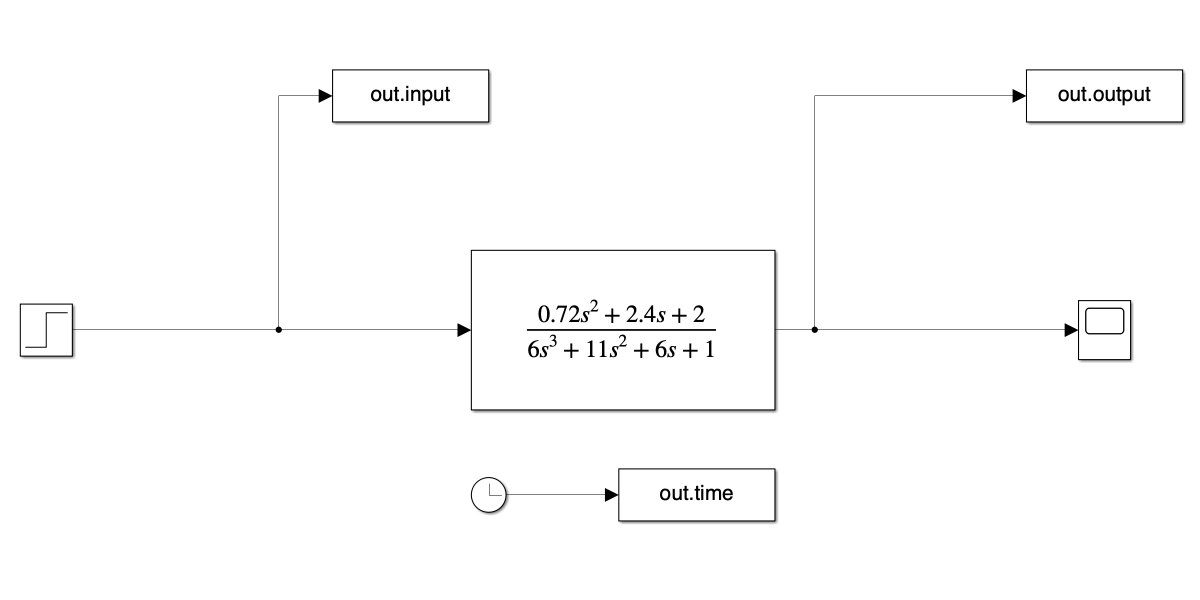
\includegraphics[width=\textwidth]{images/LSISWNIStepSimulinkModel.png}
	\caption{Simulink model with step input}
	\label{fig:LSISWNIStepSimulinkModel}
\end{figure}


\begin{code}
	\begin{matlabcode}{firstnumber = 4}
		%% Import Simulink model
		sim("LS1_1_Stp.slx")
	\end{matlabcode}
	\captionof{listing}{Importing Simulink model in Matlab}
	\label{code:LSISWNIImportStepModel}
\end{code}

The returned data from Simulink is used to calculate $\phi$ As shown in \autoref{code:LSISWNIStepResponse}. Executing this code will result in a Matlab error indicating that $\phi$ is singular and can't be inverted, which is as expected. At least three columns of $\phi$ are linearly dependent since we used the step input value to populate those columns. We can not invert $\phi$ and we can not calculate $\theta$ and identify the system in this case. \autoref{code:LSISWNIImportStepModel} and \autoref{code:LSISWNIStepResponse} are from \hspace{-1ex}\lstinline| assignment1/part1/1_1/LS1_1_step.m| and Simulink model is located at \hspace{-1ex}\lstinline| assignment1/part1/1_1/LS1_1_STP.slx|.

\begin{code}
	\begin{matlabcode}{firstnumber = 7}
		%% Prepare Data
		u = ans.input.Data';
		y = ans.output.Data';
		t = ans.time.Data';
		
		%% Calculate Phi
		N = length(u);
		phi = [-y(3:N-1)' -y(2:N-2)' -y(1:N-3)' u(3:N-1)' u(2:N-2)' u(1:N-3)'];
		
		%% Check if phi is singular
		if cond(phi)> 1e15
		fprintf(2,"phi is singular and can't be inverted.\n")
		pause(0.1)
		return
		end    
	\end{matlabcode}
	\captionof{listing}{LS with step input in Matlab}
	\label{code:LSISWNIStepResponse}
\end{code}

We can improve our approach by using a white noise with a variance of $2$ as input of the system. \autoref{code:LSISWNIInputNoiseGeneration} presents the required steps to generate the white noise input of the system.
We also modify the Simulink model to apply the generated noise input to the system as shown in \autoref{fig:LSISWNINoiseSimulinkModel}.

\begin{code}
	\begin{matlabcode}{firstnumber = 4}
		%% Generate white noise with variance of 2
		desired_variance = 2;
		signal_length = 3334; 
		standard_noise = randn(signal_length, 1);
		current_variance = var(standard_noise);
		scaling_factor = sqrt(desired_variance / current_variance);
		white_noise = standard_noise * scaling_factor;
		actual_variance = var(white_noise);
		fprintf('Desired variance of input white noise: %.2f\n', desired_variance);
		fprintf('Actual variance of input white noise: %.2f\n', actual_variance);
	\end{matlabcode}
	\captionof{listing}{White noise generation in Matlab}
	\label{code:LSISWNIInputNoiseGeneration}
\end{code}

\begin{figure}
	\centering
	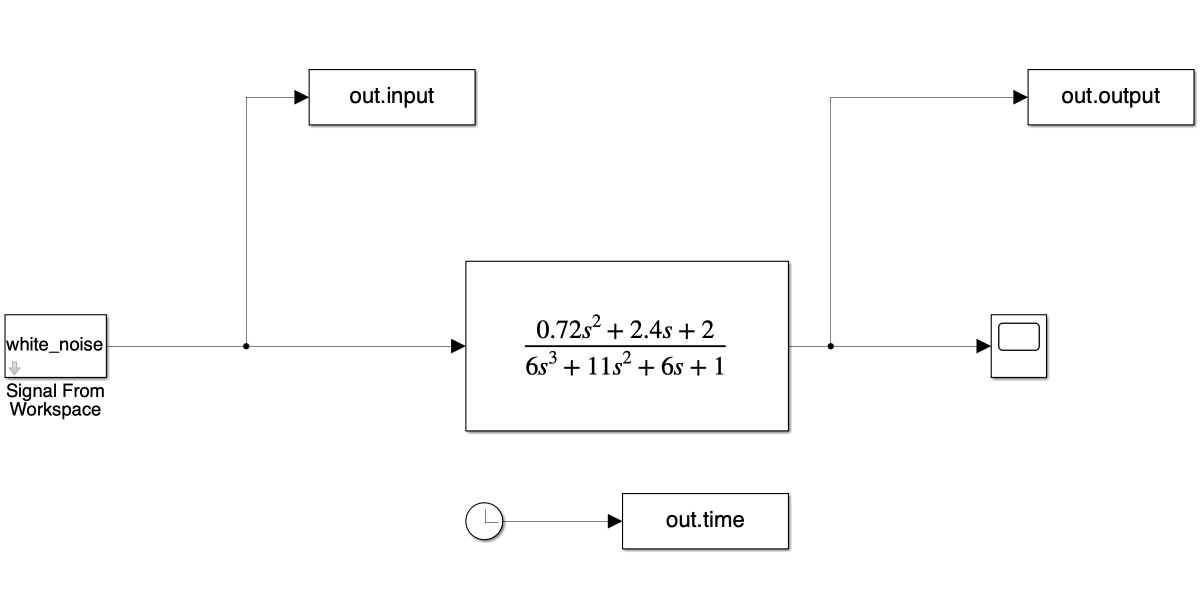
\includegraphics[width=\textwidth]{images/LSISWNINoiseSimulinkModel.png}
	\caption{Simulink model with white noise input}
	\label{fig:LSISWNINoiseSimulinkModel}
\end{figure}

\autoref{code:LSISWNINoiseResponse} outlines the remaining steps required to identify the system. \autoref{fig:LSISWNINoiseOutputVSSimulated} shows the difference between actual system's output versus the identified system's output when white noise input applied. Furthermore $\theta$ and the identified contineus system are shown in \autoref{eq:LSISWNIThetaNoiseInput} and \autoref{eq:LSISWNISystemNoiseInput} accordingly. The MSE has  $10^{-21}$ orders of magnitude which is very small and indicates our identified model closely resembles the actual system in this scenario.

\begin{code}
	\begin{matlabcode}{firstnumber = 15}
%% Import Simulink model
sim("LS1_1_NS.slx");

%% Prepare Data
u = squeeze(ans.input.Data)';
y = squeeze(ans.output.Data)';
t = ans.time.Data';

%% Calculate Phi
N = length(u);
phi = [-y(3:N-1)' -y(2:N-2)' -y(1:N-3)' u(3:N-1)' u(2:N-2)' u(1:N-3)'];

%% Check if phi is singular
if cond(phi)> 1e15
fprintf(2,"phi is singular and can't be inverted.\n")
pause(0.1)
return
end   

%% Calculate Theta_hat
Y = y(4:N)';
theta_hat = inv(phi'*phi)*phi'*Y;

%% Calculate model output and its error
YP = phi*theta_hat;
error = Y-YP;
MSE = mse(error);

%% Plot output and estimated output
y_hat = phi*theta_hat;
t=1:length(y_hat);
figure;plot(t,y(:,1:length(y_hat)),t,y_hat);fontsize( 24 ,"points");legend('Measured','Simulated');
grid on;hold on;
title("LS parameter estimation with white noise input");xlabel('Sample Number');ylabel('Amplitude');

%% Recreate system model
sysCSD = tf(theta_hat(4:6)',[1 theta_hat(1:3)'],0.3)
sysCS = d2c(sysCSD)
	\end{matlabcode}
	\captionof{listing}{LS with white noise as input in Matlab}
	\label{code:LSISWNINoiseResponse}
\end{code}

\begin{figure}
	\centering
	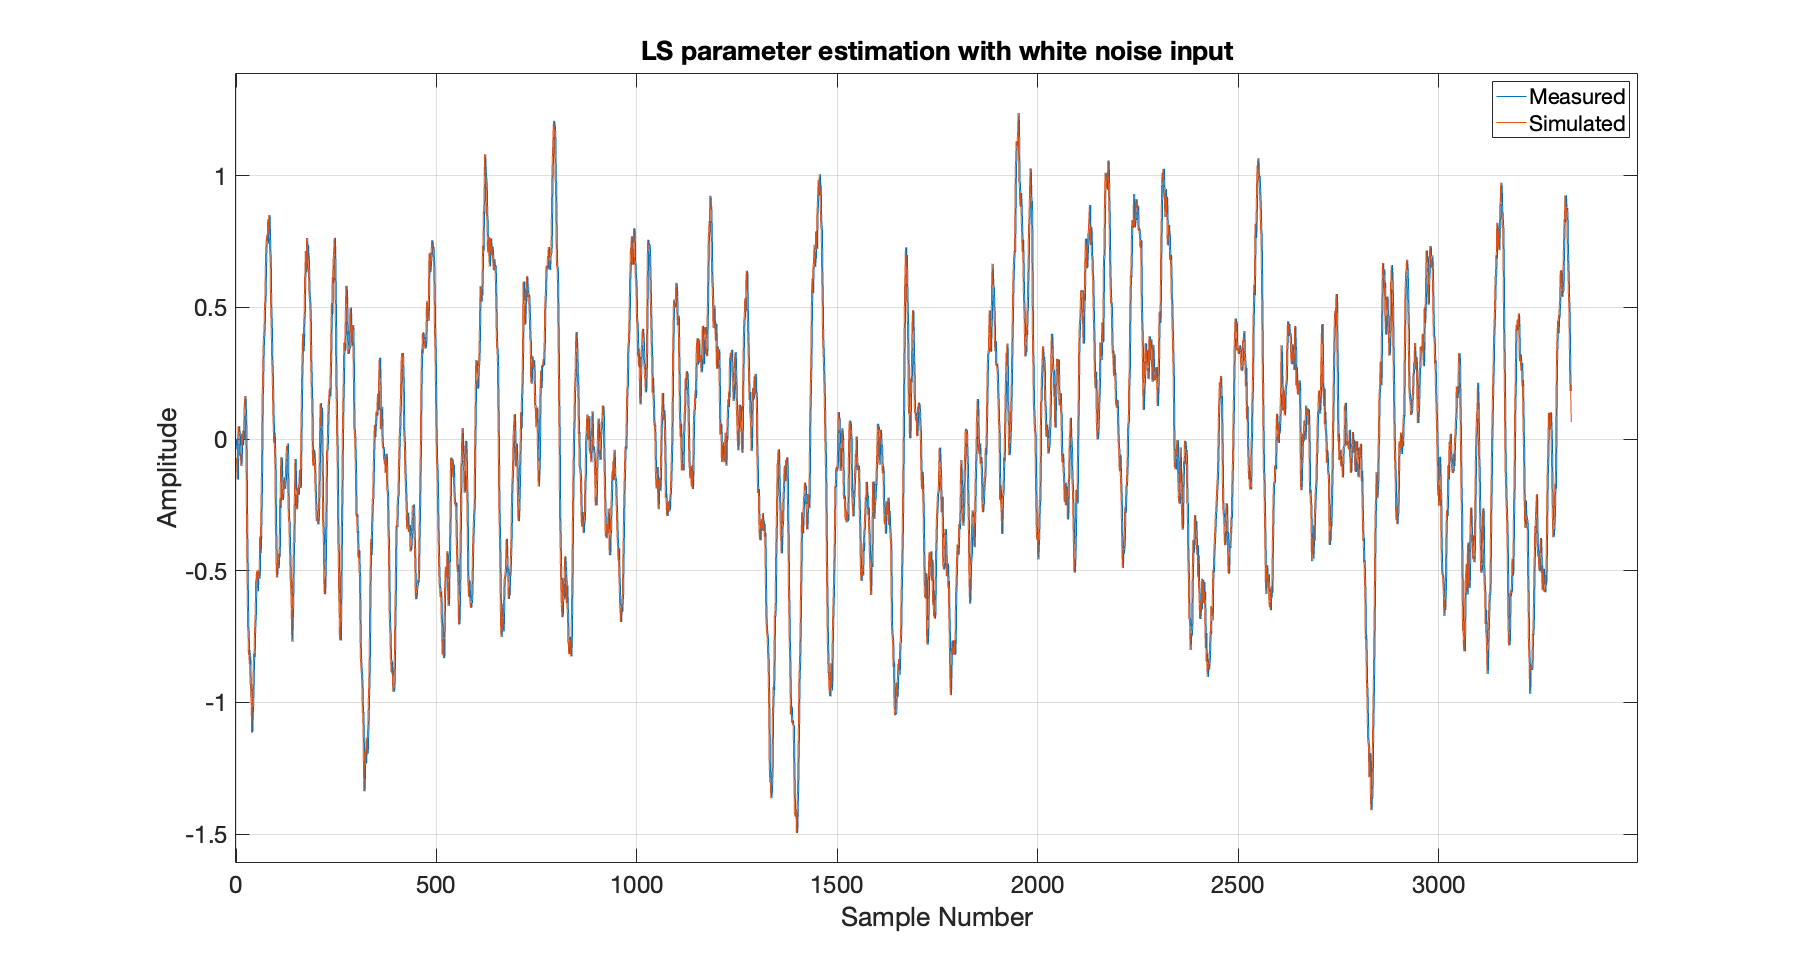
\includegraphics[width=\textwidth]{images/LSISWNINoiseOutputVSSimulated.png}
	\caption{LS system output comparison for white noise input}
	\label{fig:LSISWNINoiseOutputVSSimulated}
\end{figure}

\begin{equation}
	\begin{gathered}
		\theta^T = [-2.506; 2.086; -0.576; 0.043; -0.052; 0.015]
	\end{gathered}
	\label{eq:LSISWNIThetaNoiseInput}
\end{equation}

\begin{equation}
	G(z) =	\frac{0.04357 z^2 - 0.05249 z + 0.01579}{z^3 - 2.506 z^2 + 2.086 z - 0.5767}
	\label{eq:LSISWNISystemNoiseInput}
\end{equation}

\autoref{code:LSISWNIInputNoiseGeneration} and \autoref{code:LSISWNINoiseResponse} are from \hspace{-1ex}\lstinline| assignment1/part1/1_1/LS1_1_noise.m| and the Simulink model is located at \hspace{-1ex}\lstinline| assignment1/part1/1_1/LS1_1_NS.slx|.
